\documentclass[11pt]{article}
\usepackage{fullpage}
\usepackage{graphicx}
\usepackage{amsmath}
\usepackage{natbib} 

\title{CS63 Spring 2024\\Robot Maze Challenge: Exploring A* Search and Reinforcement Learning for Pathfinding}
\author{Kanyarin Boonkongchuen, Mark Lohatepanont, Rachel Sun}
\date{May 6, 2024}

\begin{document}

\maketitle

\section{Introduction}

% Your paper should be 4-6 pages long.  In this section you should give
% a broad introduction to your project.  Assume that you are writing to
% an audience that is familiar with AI, but may not know the details of
% the particular technique that you are using.  You should give an
% overview of the approach being explored, and how you applied it to a
% particular problem. 

The maze solving problem is looking at how to get a robot to move around a maze
to a predetermined goal that has walls as obstacles. The robot is continuously
moving according to a velocity and angle given by the controller. We want the
robot to be able to successfully navigate the maze without hitting any obstacles
and reach the predetermined goal state. To find the optimal path through the
maze we will attempt to apply an A* search algorithm and reinforcement learning
(RL) algorithm to find the best path. A* is a state space search algorithm that
uses a heuristic function plus the cost from start state to current state to
decide what state to enter next. Q-learning is a type of reinforcement learning
that uses q-values that correspond to how good a state action pair is. Once we
have found the best path, we will then try to have the robot follow that line.
Once the robot has successfully moved from the start state to the goal state,
then the problem will be considered solved.

\section{Methods}

% In this section you should explain the details about your project.

% For example, if your project is based on a Kaggle competition, this should include
% describing the data set used (number of patterns, number of features,
% description of features, any preprocessing that was necessary) and its
% source.

% You should provide all of the parameter settings used (such as
% learning rate, etc.).  You should also provide details about how the
% system was trained, and how you determined when to end training.

% Details about how to test and run your \emph{code} should NOT be given in the
% paper, but should instead be described in the README file in the lab
% directory. 

    We defaulted to using (25, 25) as our starting position and coordinates 25 pixels away from both bottom and right walls as the goal.

    \subsection{Maps}

    We created 6 black and white maps where white pixels represent open space
    and black pixels represent walls or obstacles. Initially, we created the
    maps only in dimensions of 500 x 500 pixels. However, the search space
    proved to be to big for RL, we created smaller versions with dimensions 250
    x 250.
    
    \subsection{Environment}
    We created a custom environment we created which allows operation of a robot by providing it with a world to live in. The environment is used by providing it with a map in a png format, where it converts it to a 3D numpy array corresponding to X (dim 0), Y(dim 1) and RGBA (dim 3) pixels. These pixels have two major states which are available spaces as white pixels, and walls as black pixels. 

    The environment is also responsible for managing agents within it and has a step function which steps forward the world, one unit in time and updates the active agent's position by moving each agent in their current direction by their current velocity. We also use a random offset to their velocity between 0 and 1 to simulate, at least in a minor scale, some wheel slippage and odometry difference. 

    The environment is also fully capable of rendering and showing the robots position, perception window, path to target, and target.

    Parameters: Map, start x, start y, goal x, goal y

    \subsection{Robot}
    The robot is technically a subcomponent of the environment, where the environment is able to add and remove agents and the environment interfaces to each agent by referencing their value in a list.

    The robot contains properties that determine how the environmental step function affects it. The primary controllables are a velocity, and an angle measurement. Velocity, for ease, can be set directly with a set function, while the angle is changed incrementally by a certain value. I believe this makes sense because in reality, a robot with high torque and sufficient breaking should be able to change velocity nearly instantaneously (s<0.5s), but changing direction is always incremental. 

    \subsection{Line Following Controller Algorithm}
    To control the robot through the environment, a line following controller is added to control the robot's velocity, and direction based upon the perception window of the robot. 

    To concretely define the perception window of the robot, a perception window
    is analogous to a camera on an actual robot, and is the way the robot
    perceives its surroundings. For an added challenge we chose to use this
    perception window instead of having the robot be able to directly access the
    world. The perception window is defined through two parameters, , and R.
    These parameters judge how many pixels the robot can see. 

    \begin{figure}[ht]
        \centering
        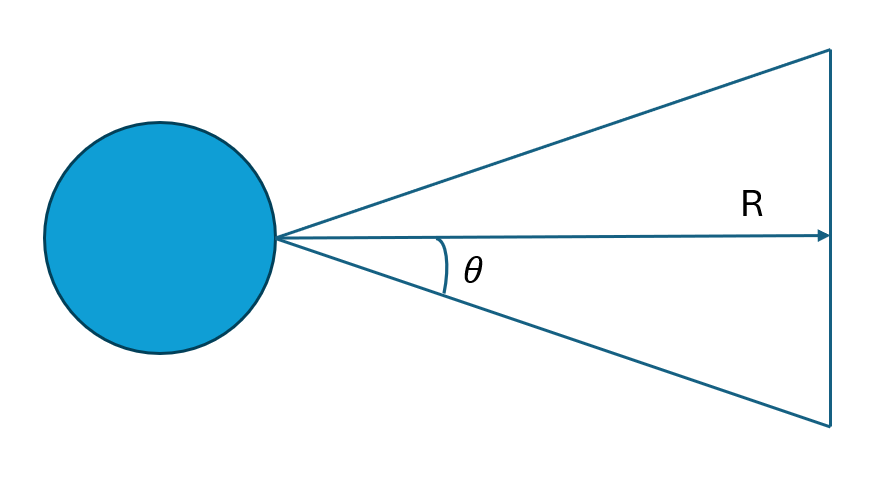
\includegraphics[scale=0.2]{figures/perception_window.png}
        \caption{Perception Window}
        \label{fig:Perception_window}
    \end{figure}
    
    To create the perception window we used a form line rastering to draw the bounding box and used it to get the pixels within this range. Keeping this window in mind, the robot is now able to see the environment around it, with particular interest in detecting the target line, which exists as a trace of points that span the entire map and plots the most efficient path from the robot's starting to ending position.

    Using the perception window we then created a controller based upon the
    error signal generated by the difference between the robots current
    direction and the targeted direction. Obtaining the error, we then
    implemented a proportional controller which takes the error signal and
    modifies it to obtain an angle correction. This is described concretely in
    Equation  \ref{eq:1}.

    \begin{equation} \label{eq:1}
        \Delta \theta = k_p e
    \end{equation}

    This controller is basic, and cannot achieve a zero steady state integrator. For future work we would likely want to add an integrator to the controller. 

    The controller exists within a large finite state machine (FSM) with two
    states, discluding initial and end states. The two states are a found line
    and line not found. This is described more concretely in Figure \ref{fig:state_machine}.
    
    \begin{figure}[ht]
        \centering
        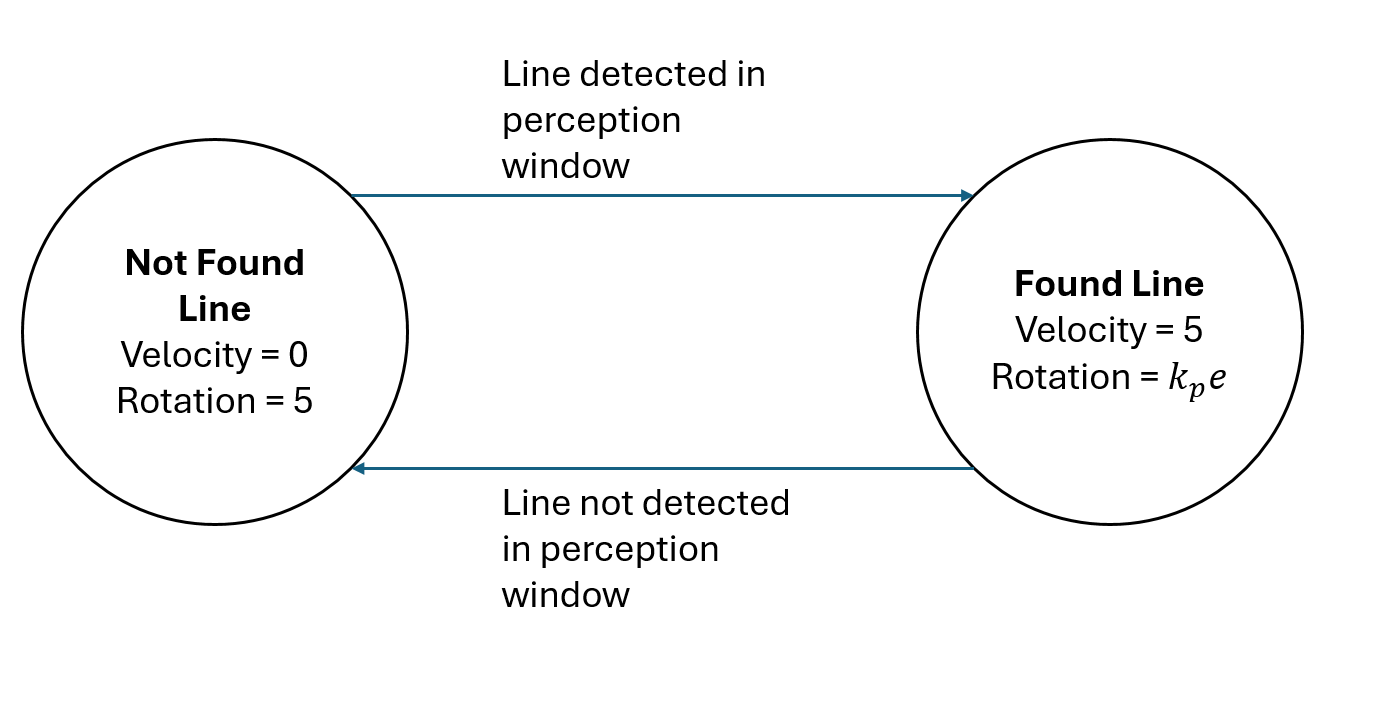
\includegraphics[scale=0.2]{figures/state_machine.png}
        \caption{State machine diagram for control scheme}
        \label{fig:state_machine}
    \end{figure}

    \subsection{A* Implementation}

    The A* algorithm works by giving priority to states based on how far they have moved from the start state plus a heuristic estimate of how far the current state is from the goal. For our implementation, A* searches by building a tree of nodes, where each node contains the parent state, current state, its depth within the tree. It checks for available moves, and expands nodes based on minimizing cost represented by the depth and the expected cost provided by our heuristic function. 

    The A* algorithm relies on having a heuristic function that should return a best estimate of how far the agent is from the goal and always underestimates the amount of steps the agent is from the goal, i.e. be admissible. By always underestimating the distance to the goal, we can guarantee an optimal solution because in the worst case, we will check every possible path to the goal before getting to the shortest path. But if we happen to overestimate the cost of that path, then we may possibly choose a suboptimal path that has a lower estimated cost.  And as long as the heuristic does not overestimate the distance to the goal, the search algorithm will always return the best possible path to the goal. 
    
    Our heuristic function: The heuristic function that we used for our implementation of A* is the euclidean distance from the current state of the robot to the goal state. We can use the pythagorean theorem to find this number using the equation below: 

    \[ H = \sqrt{(current_x-goal_x)^2 + (current_y - goal_y)^2}\]

    This heuristic will always be less than or equal to the amount of steps we
    still need to take to get to the goal state because the shortest path from
    one state to another is to move along the diagonal. This diagonal is
    calculated by the equation above which guarantees that our heuristic will
    return something that is always less than or equal to the actual steps
    needed to get to the goal. 

        \subsubsection{State Space}

        In A*, the state space for the maze problem is a set of coordinates (x, y) that represents the current location of the robot on the map. 

        \subsubsection{Action Space}

        The action space has a maximum of 8 moves available at any state: moving
        one pixel in the 8 cardinal and ordinal directions (N, NE, E, SE, S, SW,
        W, NW). If the next state is a wall, represented by black pixels, the
        move is not considered a possible move. In addition, in order to ensure
        that the path that A* algorithm produces is not to close the walls (to
        avoid crashing when we have a controller followed the path), we perform
        the A* search on an inflated map, which increases the width of the walls
        by 20 on each side. Therefore, moves too close to the walls are also not
        considered as possible moves. 

        \subsubsection{Goal}

        The problem is considered solved when the current state equals the goal state. 
    
    \subsection{RL Implementation}

    A RL algorithm works by having an agent explore the environment and simultaneously calculate a table of values, called a q-table, that learns how good a certain state-action pair is. There are rewards associated with each possible state and the q-value equation takes the rewards into account when updating the q-value, which represents the expected future reward by moving to that particular state. The q-table is learned as the agent explores the environment which gradually updates the q-table using temporal difference learning. During the learning process, the agent picks action using epsilon greedy action selection.

    Epsilon greedy action selection is done by using a pseudo-random number
    generator to generate a number between 0 and 1. If the number is less than
    our current epsilon value, then we will take a random possible action from
    the current state as our next move. Else, if our random value is more than
    or equal to the current epsilon value, then we will take the greedy action
    or the action with the best possible current q-value out of all the possible
    actions we could take. Then after each step in our learning process, we then
    decay the value of our epsilon by a set factor to make it smaller than
    before up to a certain extent. This means that in the beginning we will pick
    random actions more than greedy actions and then we will slowly transition
    into picking more and more greedy actions over time. The starting epsilon
    value, minimum epsilon value, and epsilon decay value are all tunable
    hyperparameters that can be changed to meet the specifications of each
    problem.
    
        \subsubsection{Q-Table Implementation}

        Once we have picked an action, we need to update our q-table with new values. The equation we are using to update the q-table values is as follows:

        \[ \text{Value}\ = (1- \alpha)*q(s,a) + \alpha * (\text{reward} + \gamma
        *\text{max a \{ } q(s_{s+1},a_{s+1}) \})  \]



        \( q(s,a)\) is the q-value of the current state and action and \(
        q(s_{s+1},a_{s+1})\) is the q-value for the state and action that is one
        step away from our current state and action. \(\alpha\) denotes the
        learning rate, and \(\gamma\) denotes the discount. Reward comes from
        the reward value of the current state we are at. And alpha and discount
        are tunable hyperparameters that can be tuned to meet the requirements
        of each different problem. 

        In this implementation, we also implemented a version that uses a neural network to learn the weights instead of the q-table using a similar equation. This implementation was also focused on finding a path that our robot could traverse on. 

        Once the learning is complete, a path is constructed by first starting
        at the start state, then we pick each subsequent state using the greedy
        selection strategy, until, hopefully, the goal state is reached. 

            \paragraph{State Space} 
            Same as A*, the state space is a set of coordinates (x, y) that represents the current location of the robot on the map. 

            \paragraph{Action Space}
            The action space has a maximum of 8 moves available at any state: moving
            one pixel in the 8 cardinal and ordinal directions (N, NE, E, SE, S, SW,
            W, NW). Unlike A*, all moves no matter if the next state is a wall are
            considered possible moves. 

            \paragraph{Goal}
            The problem is considered solved when we create a q-table that can be used to construct a path from the start state to the goal state. 

            \paragraph{Reward} 
            Because we projected RL to take substantial time to run and with
            consideration of the time constraints of the project, rather than
            assigning the award only at the goal, a table of rewards is created
            before beginning the search. The reward table has the same dimension
            as the map to represent the immediate reward at each state of the
            map. Rewards are calculated from the goal position expanding outward
            using depth first search, with the highest reward value at the goal
            and descending values outward in the subsequent states. Then, a
            reward of -100 is assigned at states on and near the walls of the
            map to lower the probabilities of the agent from constructing the
            path near them. 

            Table \ref{table:1} displays the values for hyperparamters we set
            for Q-table.

            \begin{table}[h!]
                \centering
                \begin{tabular}{|c c|} 
                \hline
                hyperparamter & value  \\ [0.5ex] 
                \hline
                epsilon & 1 \\
                epsilon decay & 0.999 \\
                epsilon min & 0.999 \\
                discount & 1 \\ 
                alpha & 0.1 \\ [1ex] 
                \hline
                \end{tabular}
                \caption{hyperparameter values for Q-table implementation}
                \label{table:1}
            \end{table}
        
        \subsubsection{Deep-Q local information implementation}

        In this version, instead of finding a path to the goal using RL, we
        directly moved the robot using values generated by RL. The robot is
        controlled by a velocity and angle so in this version, we implemented a
        neural network that would learn to predict what angle the robot should
        move at, given a point on the map. The model is trained by running the
        robot from the starting position numerous times with the model giving
        angles to move the robot. If the robot crashes into a wall or reaches
        the goal, the run ends and the environment and robot are reset to the
        starting position and then we run again. Every so often we will do a
        batch sample of our previous runs to train the model with the data we
        have collected. 

            \paragraph{Model} We used the model from Lab 8. To match our
            problem, we changed the input number to 2 and the output number to 9. 

            \paragraph{State Space}
            Same as A*, the state space is a set of coordinates (x, y) that represents the current location of the robot on the map. 

            \paragraph{Action Space}
            The action space is a discrete list of angles that the robot could move at. For this we set them to be: -8, -5, -3, -1, 0, 1, 3, 5, 8

            \paragraph{Rewards}
            The rewards are set at the goal state. If the robot reaches the goal
            state, it will be rewarded 1000 points. If the robot crashes into a
            wall, it will receive -500 points. And for every step the robot
            takes without crashing, it also accumulates 1 point per step. This
            is to encourage the robot to go as long as possible without
            crashing. 
            
            \paragraph{Goal}
            The problem is considered solved when the model we create from RL is able to guide the robot through the maze and reach the goal state without crashing.

        Table \ref{table:2} displays the values for hyperparamters we set for Deep-Q.

        \begin{table}[ht!]
            \centering
            \begin{tabular}{|c c|} 
            \hline
            hyperparamter & value  \\ [0.5ex] 
            \hline
            epsilon & 1 \\
            epsilon decay & 0.99 \\
            epsilon min & 0.3 \\
            discount & 0.9 \\ 
            alpha & 0.1 \\ [1ex] 
            \hline
            \end{tabular}
            \caption{hyperparameter values for Deep-Q implementation}
            \label{table:2}
        \end{table}

\section{Results}

% In this section you should show and analyze the results.  Measure the
% performance of your system, and if possible compare your performance
% to other implementations. Use tables and figures to illustrate the
% results.  You should also discuss what sorts of conclusions can be drawn from
% these results; what did you learn, what are the important takeaways for a
% reader, etc.

% Even if your project is not as successful as you'd hoped, you still
% need to show and discuss results.  This section is one of the key parts of any
% scientific paper.  Be sure to provide adequate information so that the
% reader can evaluate the outcomes of your experiments. 

    \subsection{Controller}
    The controller is able to navigate to the goal with a path that is not too
    close to the walls and reaches the goal. This can be seen in Figure
    \ref{fig:map4_robot}.

    \subsection{A*}
    Our implementation of A* search is able to successfully find the optimal
    path to the goal in the 6 500 x 500 we created . Figure \ref{fig:map4_path}
    shows the resulting path plotted on Map 4. As intended by
    using an
    inflated version of the initial maps, the paths are a some distance away
    from the walls of the mazes.

    \begin{figure}[ht]
        \centering
        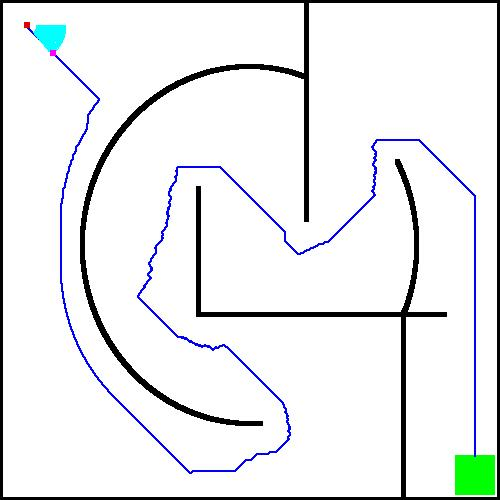
\includegraphics[scale=0.2]{figures/map4_start_world_6.jpg}
        \caption{Path plotted by A* on 500 x 500 Map 4}
        \label{fig:map4_path}
    \end{figure}

    \begin{figure}[ht]
        \centering
        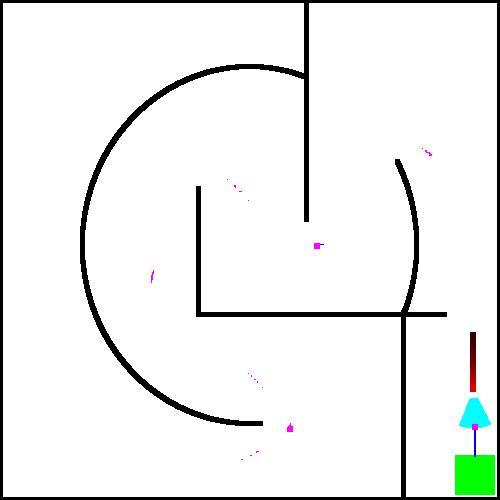
\includegraphics[scale=0.2]{figures/map4_end_world_504.jpg}
        \caption{Robot following path in Figure \ref{fig:map4_path} }
        \label{fig:map4_robot}
    \end{figure}


    \subsection{RL}

        \paragraph{Q-Table global information implementation}
        This implementation of RL did not work as expected. For most trials, it was not able to find a path to the goal and often ended up making either a straight line into a wall, or going around in circles around the starting point.
        
        \paragraph{Deep-Q global information implementation}
        The second implementation also fails to find a path to the goal. In trials with 1000 episodes and 1000 steps per run, the agent often plots a straight horizontal line from the starting position into the right wall. 

        \paragraph{Deep-Q local information implementation}
        We observed significant improvement in our third implementation when testing on the 250 x 250 Map0, the blank map with only outer walls. For Maze0, in trials with a couple thousand episodes and with 1000 steps per episode, the robot is able to generally move toward the goal’s direction and reach it during testing. However, the robot tends to make a few loops and stray away from the optimal direction in the process.

        Positive results end there, however. When testing on Maze 1 with actual mazes with walls using the same hyperparameters as our tests on Maze0, the robot fails to find the goal. In trials in 250 x 250 Maze1, the robot moves in a horizontal direction from the starting position for a bit of distance, a visual estimate of about 25 pixels, before veering from the initial direction crashing into the wall. Tests on 250 x 250 Maze 2 yielded similar performance, where the robot is only moved stably horizontally for about a distance before veering and crashing. 

        Due to time constraints and the poor performances on Maze1 and Maze2, we did not conduct further testing on the rest of the available maps. 

\section{Discussion}
    \subsection{Controller}
    A constraint that the current controller has is that the plotted path has a
    sharp turn, such as in Maze, the robot momentarily has no path points within
    its perception window. Essentially, it loses sight of the path, and would
    have to adjust by defaulting to turning in place searching for the path. 
    
    The previous can be patched by having the robot stay stationary and turn to
    look for the following points. However, the root cause of the problem for
    line following with uncertain velocity is that the proportional controller
    does not take into account the error that builds up within a system. This
    problem is shown in figure 3 where a proportional controller can never reach
    a desired angle.
    
    Figure \ref{fig:prop_controller} highlights that without an integrator, the
    error will continuously oscillate around the desired angle and this leads to
    error that builds up over time. To obtain correct tracking a proportional
    integral derivative controller may be more beneficial to use, however that
    is also excessive. Technically, a robot like this which we only directly
    control the angle’s rotation by increasing the angle by a linear amount (we
    can constrain angle movements to a arbitrary value like 2 degrees per
    iteration), is a second order laplace system with a transfer function of
    form \( 1/(s^2+as+b) \). This indicates that an proportional integral or PID
    controller will be sufficient for full control with zero steady state error.

    \begin{figure}[ht]
        \centering
        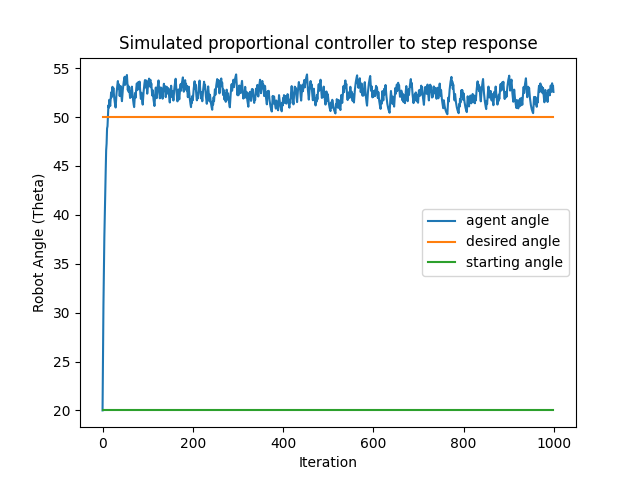
\includegraphics[scale=0.4]{figures/Sample proportional controller error.png}
        \caption{Sample proportional controller error}
        \label{fig:prop_controller}
    \end{figure}

    \subsection{A*}
    The A* search worked pretty well and always found the best path to the goal that the robot is also able to follow. One way we could improve this would be to make a better heuristic function that takes into account the walls that are blocking the way. This would make the A* better at picking a path to go and reduce the amount of time that the A* takes to find the best path. Currently we are using euclidean distance to the goal which does not take into account the walls at all although it is also guaranteed to underestimate, it may severely underestimate which would mean we have to explore more nodes. A better heuristic would be closer to the actual steps needed to the goal. This may be able to be done by adding a step for every wall pixel found within the line created by euclidean distance. In addition, to make it easier for the robot to follow the line that we would eventually create, it would have been nice if we could have made the line have less sharp turns because the robot really struggles with getting around sharp corners. This slows the robot down considerably when it needs to turn in place to find the line again after it loses sight of it. For the robot not to do this, it would have been great if we could modify A* search further to produce a line that makes a wider turn around corners. This would also allow the robot to move at higher velocities as right now, it moves pretty slowly to give it enough time to turn before it will crash.

    \subsection{RL}

    We rescaled the map to be smaller to see as we suspected that the original 500 x 500 dimension is too big for RL to run in the time that we had. And even with a smaller map, training time proved to be too long to produce a set of weights that reached the goal. 

    In our initial implementation of RL, we opted to use a q-table. Q-table required exploring the maps quite thoroughly in order to produce viable results. Thus, we thought to assign rewards with global information on the map in an effort to expedite the search process. Although we did assign negative rewards on walls, our reward assignment strategy does not take into account dead ends that exist in the map. As a result, we speculate it is possible that there are states which can have high q-values, which can make the robot falsely think this is a good state. And since in this scenario we have global information, there is probably a more sophisticated way we could have assigned rewards in order to make the robot perform the best in the shortest possible amount of time.

    While training Deep-Q local information implementation, we load weights found in previous trials in order to continue to progress from previous training. A noticeable difference between each test in which we load newly found weights when testing on 250 x 250 Maze1, is that the robot seems to move in a straight line farther with each trial before veering randomly and crashing into the wall. This shows that it might have reached the end of the area where it has explored in training and now doesn’t know what to do anymore when it reaches somewhere new. But this suggests that more training time could help with this as the robot would be given more time to explore all of the different states and figure out what to do in these new scenarios. 

    \subsection{Compare A* \& RL}
    RL takes a long time to train compared to A* search. Our implementation of A* was able to find the best path for a larger map when compared to RL where even in a smaller map, it couldn’t successfully find the goal. However, A* needs global information to be able to give us this very fast time and optimal path guarantee. This may not be possible in many applications so RL may be a better choice if we cannot get global information. However, RL takes a really long time to train and the weights cannot be applied to a new map so each map will need to be retrained 


\section{Conclusions}

% This section should sum up what you did and what you found.  It is also
% appropriate to mention things you would have liked to do but didn't have time
% for as `future work.'

In this paper, we have explored several methods of getting a robot to solve a
maze. We were able to do this with varying degrees of success as described in
the paper. The A* search algorithm was successful according to the goal that we
set up in the beginning but it requires global information which is not always
readily available. While the RL implementation does not require global
information, the training time required to reach the goal proved to be too long
for us to be able to see good results. We hoped that we could have had more time
to finish training and polishing our RL implementation, but given the scope of
this project and the time given for it, it wasn not feasible to polish RL to a
working state. Since the mazes we design had a couple false paths that would
lead to dead ends, the RL would have to take time to explore all of those paths
to be able to determine they do not lead to the goal. The RL implementation
showed promising signs that a longer training time would lead to a better
result. We are also constrained by the computer resources that were available to
us and did not have the time to be able to compensate for that. If we were to
continue this project, we would like to train the RL algorithms for longer to
see if it can improve its performance. With more time, we would also be able to
test the algorithms on maps we have not tested on and on bigger maps. 

\section{Acknowledgements}

% You should clearly acknowledge any outside sources of help you had.  In
% particular, if you used resources from the internet, you should describe what
% they were and how they were used.  Note that this applies to all phases of the
% project, including coding, analysis, and writing.  This doesn't need to be
% long, but should include enough detail it's clear what you did yourself and
% what you got from elsewhere.

% For instance, you might say that you got help brainstorming and finding good
% libraries to use from Professor A, then got help figuring out how to apply
% statistical tests from Professor B, and finally used ChatGPT to generate an
% outline for the `Introduction' section.
We would like to thank Professor Ben Mitchell for helping us with this project.

\section{References}

\noindent

Mitchell, B. (2024) \textit{Lab 1: Controlling a robot in a maze} Available at https://www.cs.swarthmore.edu

/mitchell/classes/cs63/s24/labs/00.html (Accessed on 6th May 2024)


Mitchell, B. (2024) \textit{Lab 2:  Traffic Jam} Available at https://www.cs.swarthmore.edu

/mitchell/classes/cs63/s24/labs/01.html (Accessed on 6th May 2024)


Mitchell, B. (2024) \textit{Lab 8: Deep Q-Learning} Available at https://www.cs.swarthmore.edu

/mitchell/classes/cs63/s24/labs/07.html (Accessed on 6th May 2024)

% It's important to have a bibliography that gives properly-formatted citations
% to sources you used.  You can pick whatever style you want (APA, MLA, IEEE,
% etc.), but pick one and follow it correctly.

\end{document}
